For robots to become widely accessible, users have to be able to command them by specifying high-level behaviors, not by programming low-level robot controllers.
This has recently become possible by applying tools and ideas from the formal methods and hybrid systems to robotics. The resulting methodologies translate high-level tasks to discrete and subsequently low-level continuous controllers in a correct-by-contstruction manner \cite{}.
\emph{Reactive} approaches are of particular interest, since they account for a dynamic, and possibly adversarial, environment. For example, the framework in \cite{KGFP_TRO09} takes a logic formula that contains the mission specification, and by solving a two-player game between the robot and its environment, outputs a hybrid controller that is guaranteed to accomplish the mission. Other reactive approaches have been proposed in \cite{Wongpiromsarn2010} and, more recently, in \cite{Belta2013RSS}.

However, the initial approaches operate under the closed world assumption, whereas robots have moved from the reclusive workspace of the assembly line to the highly unstructured site of the Fukushima Daiichi nuclear disaster. 
Thus, there is a need for high-level robot controllers that adapt to the discrepancies between the robot's model of the world and reality. 
In addition, robots are also asked to incorporate new functions during execution. 
Examples include reconfigurable modular robots, as well as robots that learn on-the-fly \cite{SaxenaIJRR2012} or inquire online knowledge repositories \cite{rapyuta2013}. 
Finally, new mission requirements may be added after the robot has been deployed, as in the case of robotic search and rescue tasks \cite{MatthiasAI2010}, personal robots \cite{}, and autonomous space and planetary exploration missions \cite{spaceXplore2006}. 
%Uncertainty and partial a priori knowledge are inherent aspects of future robot missions, not problems that we should attempt to avoid encountering.

For example, consider the setting where a robotic courier (mailbot) is used to deliver mails in a school or company building (see Fig. \ref{Fig:pr3}). It is tasked with collecting letters and delivering them to the recipients' offices. 
This mission is relatively simple, and yet the robot's world is already open with respect to (w.r.t.) letters addressed to recipients the robot does not know about. % Na to kana entelws nia-nia dew?
Even if all possible recipients, and the locations of their offices, are fixed, the information may not be available a priori.
%\begin{myExample}\label{Ex:mailbot1} Autonomous Mailbot (Fig. \ref{Fig:pr3})\\
%	A robotic courier (mailbot) operates within a school or company building. It is tasked with collecting letters and delivering them to the recipients' offices. Even if all possible recipients, and the locations of their offices, are fixed, the information may not be available at the time the mission specification is defined.
%\end{myExample}

\begin{figure}[ht]
	\centering
	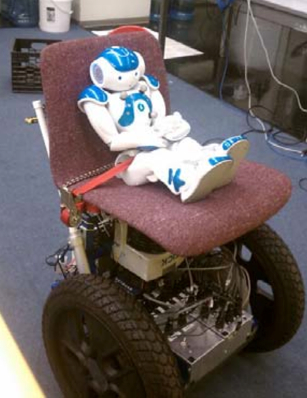
\includegraphics[width=0.7\columnwidth, clip]{./img/pr3.jpg}
	\caption{Our implementation of a mailbot. A Nao humanoid robot (ref ???) is mounted on a segway platform. The actuation and perception capabilities of the former are complemented by the localization, navigation and mobility advantages of the latter.}
	\label{Fig:pr3}
\end{figure}

However, in order to design provably-correct open world planners, a number of challenges have to be overcome. 
First, there is the assumption that a robot has full knowledge of the structure of its workspace. This issue has been tackled in \cite{MurrayICRA2012} and \cite{MurrayICRA2013a}, where the authors introduced local re-synthesis as a way to account for local topological changes in the robot's workspace. 
An approach that addresses the unreactive equivalent of the same problem appeared in \cite{Dimos2013ICRA}. 
However, the previous papers still assume that the size of the workspace is known; that only its internal structure changes. Moreover, they do not account for augmenting the mission with additional objectives, a situation which may arise if the robot can discover new regions of its workspace, or new objects of interest. 
The work in \cite{BingxinRSS2012} addresses possible additions to the robot's workspace without enforcing a known workspace size, but once again the solution is limited to changes in the spatial components of the state space. 
A true open world planner must be able to adapt to changes in other parts of the robot's world model as well, such as available sensors and actions. 
Finally, open-world planning introduces the challenge of enabling users to specify tasks over a world that is at least partially unknown prior to execution. The specification language and abstractions necessary for this have been approached with both semantic \cite{Joshi2012, MatthiasAI2010} and statistical \cite{Tellex2011} methods, but so far no solution provides the guarantees on behavior that a formal, correct-by-construction system is capable of. 

In this paper, we generalize the approach in \cite{BingxinRSS2012} to open worlds where the entire state-space may grow, not just the workspace. 
To this end, we first introduce new abstractions that allow us to specify missions without explicitly referring to individual variables (propositions). This allows the specification to be updated as new elements are discovered. These new elements can be new robot actions and environment variables, in addition to newly discovered regions of the world. 
Then, we show how the mission specification can be systematically and automatically re-written in order to correctly incorporate the new elements of the open world. We achieve that by augment a specification with elements of first-order logic.

The paper is organized as follows: Section \ref{preliminaries} provides the necessary background information on logic-based reactive mission planning. Section \ref{problem} presents the problem and its motivation, and introduces an example that we will be revisiting throughout the paper. The proposed abstractions, which we will use to specify tasks over open worlds, are treated in Section \ref{abstractions}. Section \ref{openworld} presents our approach to open world mission planning. Simulation examples of open world robot missions are given in Section \ref{simulation}. Finally, our conclusions, as well as suggestions for future work, are summarized in Section \ref{conclusion}.

% END

%Use some ideas from \cite{open-world-sw} when talking about open world:
%\begin{itemize}
%	\item Software should react to changes by self-organizing its structure and self-adapting its behavior.
%	\item Closed software: composed of parts that don't change during execution.
%	\item Changes in the world make new components available. System can discover and bind such components dynamically while the application is executing.
%	\item In practical cases, not all requirements can or should be specified upfront. Stakeholders add new requirements during execution. For example, scientists on the MARS Rover team bla bla bla (little a priori knowledge, not continuous interaction with the robot, also teleoperation slow, etc).
%	\item Uncertainty and partial a priori knowledge are inherent aspects of missions, not problems that we should attempt to avoid encountering.
%\end{itemize}